\paragraph*{Objective} \hfill \\
The objective of this experiment is to use a multimeter for measuring the resistance, current and voltage. In this exercise we should learn how a resistor influences a circuit and what its purpose is; mainly effects the voltage and the current outputs, and the other way around. Also, we should understand how to read the color codes of resistors and how to combine them in parallel and in series. 

\paragraph*{Results and procedure} \hfill\\
To find out what resistance a resistor has we looked at its colour coding, and calculated the resistance from there (brown, green, orange, gold $= 15k\Omega$ with 5\% tolerance) After identifying the resistor, it is smart to check if it actually works or not. This can be done by measuring the resistance with a multimeter.  
\begin{itemize}
\item Measurement on a $15k\Omega$ resistor shows: $14.98 k\Omega$
\end{itemize}
Conclusion. Looking at the colour coding we could see that the resistor has a tolerance of 5\%. Hence, the measured value is perfectly acceptable. In order to see how the resistor influences the current we set the voltage to 5V. To measure the voltage in the circuit, the multimeter was connected in parallel. To measure the current, we put the multimeter in series. On the side, we made calculations to later be able to compare our measurement to the datasheet. The representation of the measurements and the calculations can be seen in "Table 1." and "Table 2." respectively.
\par "Step 2" was repeated, but this time for 11 different voltages, ranging from -15 to 15V:
% add Table 1 [done] and 2 [to be]
% add calculations (V=iR)
% add plot [done]
\begin{table}[H]
	\centering
	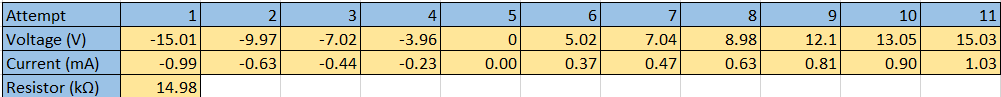
\includegraphics[width=1\textwidth]{./images/Kacper/11.png}
	\caption{Current (I) Measurement}
	\label{Current Measurement}
\end{table}

\begin{table} [H]
	\centering
	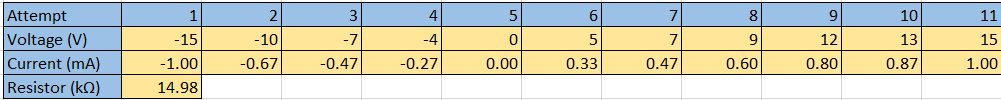
\includegraphics[width=1\textwidth]{./images/Kacper/11a.png}
	\caption{Current (I) Datasheet}
	\label{Current (I) Datasheet}
\end{table}

\begin{figure} [H]
	\centering
	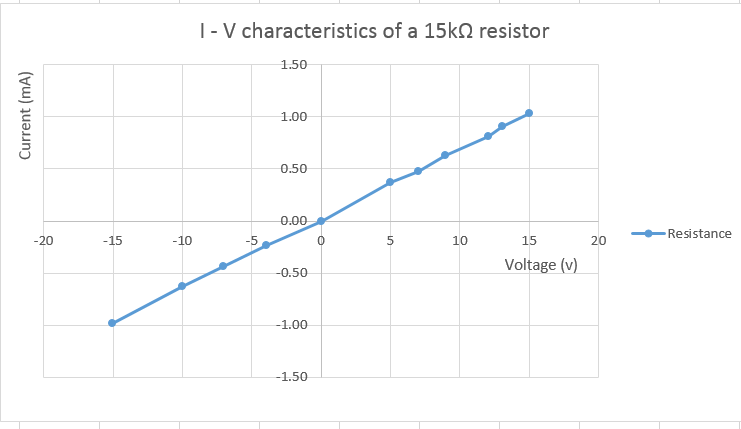
\includegraphics[width=1\textwidth]{./images/Kacper/11p.png}
	\caption{I-V Characteristics of a 15k resistor}
	\label{I-V Characteristics of a 15k resistor}
\end{figure}

\paragraph*{Conclusion} \hfill \\
In conclusion we can say that our measurements are on one line, taking the tolerance level (our margin of error) into consideration. The function is linear. We proved the Omh's Law that resistance is dependant on voltage and current.